\documentclass[tikz,border=10pt]{standalone}
\usepackage[T1]{fontenc}
\usepackage{helvet}
\renewcommand{\familydefault}{\sfdefault}
\usepackage{amsmath,amssymb}
\usepackage{tikz}
\usetikzlibrary{calc,positioning,fit,arrows.meta,shapes.geometric}

% Canonical Academic Palette
\definecolor{OxfordNavy}{HTML}{1E293B}
\definecolor{SlateSteel}{HTML}{334155}
\definecolor{MutedTeal}{HTML}{0F766E}
\definecolor{TealL0}{HTML}{F0FDFA}
\definecolor{Burgundy}{HTML}{991B1B}
\definecolor{BurgundyL0}{HTML}{FEF2F2}
\definecolor{WarmOchre}{HTML}{92400E}
\definecolor{OchreL0}{HTML}{FFFBEB}
\definecolor{ForestSage}{HTML}{166534}
\definecolor{SageL0}{HTML}{F0FDF4}
\definecolor{CoolParchment}{HTML}{F8FAFC}
\definecolor{SlateRim}{HTML}{CBD5E1}
\definecolor{GridGray}{HTML}{E2E8F0}
\definecolor{DarkSlate}{HTML}{0F172A}

\begin{document}
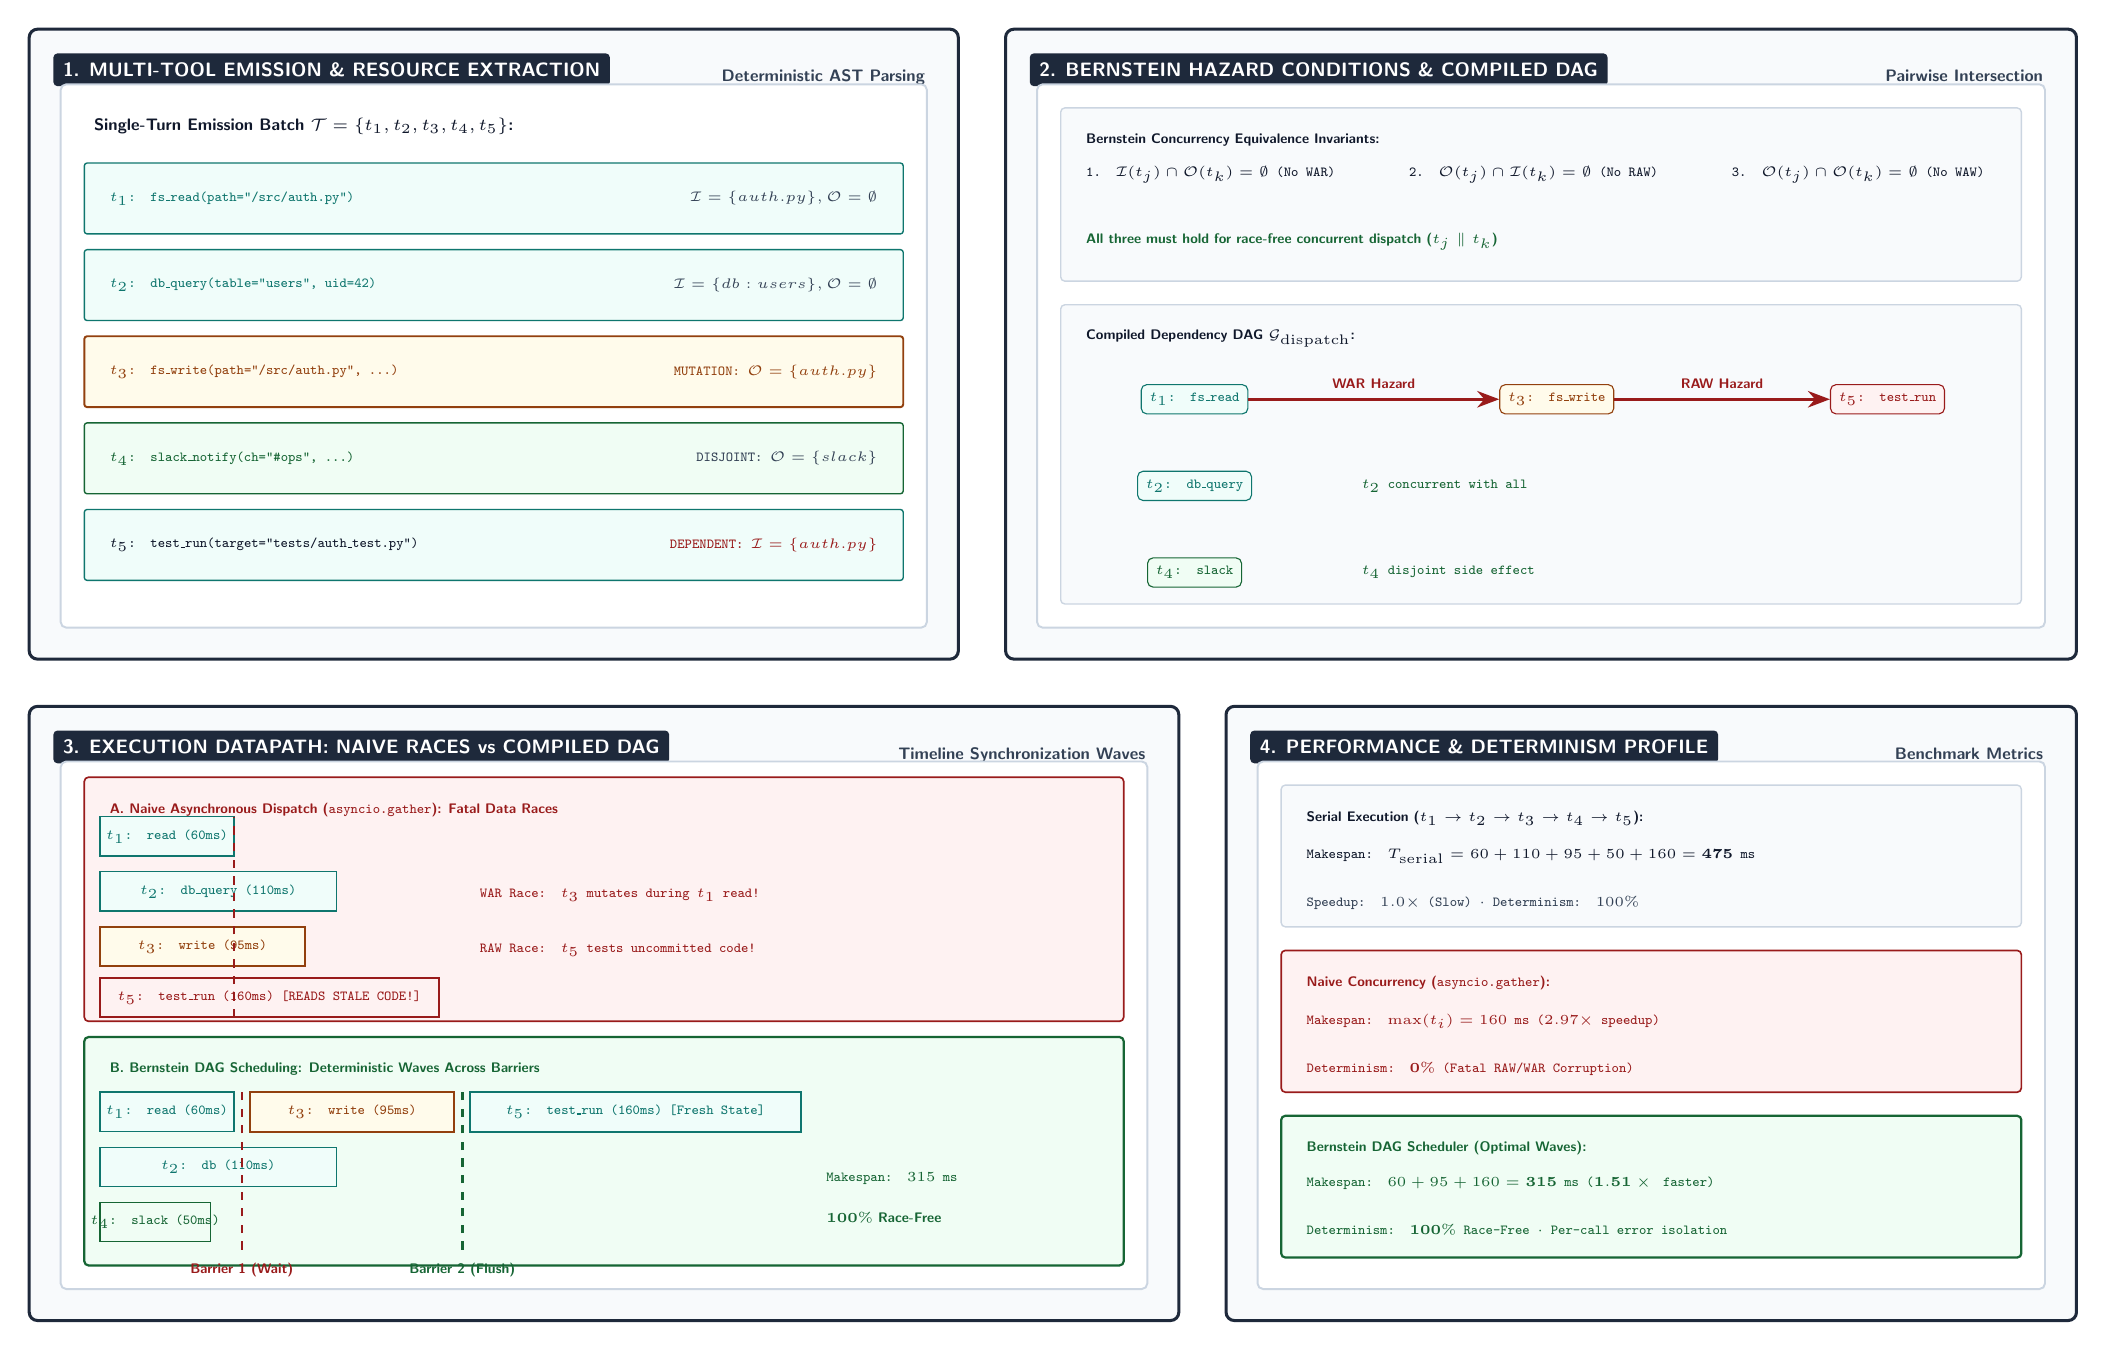
\begin{tikzpicture}[
  font=\sffamily,
  scale=1.0,
  >=Stealth,
  node distance=0.5cm
]

% =============================================================================
% TOP-LEFT (PANEL 1): TOOL EMISSION BATCH & FORMAL RESOURCE SETS
% =============================================================================
\begin{scope}[shift={(0, 8.4)}]
  \draw[fill=CoolParchment, draw=OxfordNavy, line width=1.1pt, rounded corners=3pt]
    (0, 0) rectangle (11.8, 8.0);

  \node[anchor=north west, fill=OxfordNavy, text=white, font=\fontsize{7.5}{9.0}\selectfont\bfseries, rounded corners=1.5pt, inner sep=3.5pt]
    at (0.3, 7.7) {1. MULTI-TOOL EMISSION \& RESOURCE EXTRACTION};
  \node[anchor=north east, text=SlateSteel, font=\fontsize{5.8}{7}\selectfont\bfseries]
    at (11.5, 7.6) {Deterministic AST Parsing};

  \begin{scope}[shift={(0.4, 0.4)}]
    \draw[fill=white, draw=SlateRim, line width=0.7pt, rounded corners=2pt] (0, 0) rectangle (11.0, 6.9);

    % Tool batch header
    \node[anchor=north west, font=\fontsize{5.8}{7}\selectfont\bfseries, text=DarkSlate] at (0.3, 6.6) {Single-Turn Emission Batch $\mathcal{T} = \{t_1, t_2, t_3, t_4, t_5\}$:};

    % 5 Tool Rows
    % t1
    \draw[fill=TealL0, draw=MutedTeal, line width=0.5pt, rounded corners=1pt] (0.3, 5.0) rectangle (10.7, 5.9);
    \node[anchor=west, font=\fontsize{4.8}{5.5}\selectfont\bfseries\ttfamily, text=MutedTeal] at (0.5, 5.45) {$t_1$: fs\_read(path="/src/auth.py")};
    \node[anchor=east, font=\fontsize{4.5}{5.2}\selectfont\ttfamily, text=SlateSteel] at (10.5, 5.45) {$\mathcal{I}=\{auth.py\}, \mathcal{O}=\emptyset$};

    % t2
    \draw[fill=TealL0, draw=MutedTeal, line width=0.5pt, rounded corners=1pt] (0.3, 3.9) rectangle (10.7, 4.8);
    \node[anchor=west, font=\fontsize{4.8}{5.5}\selectfont\bfseries\ttfamily, text=MutedTeal] at (0.5, 4.35) {$t_2$: db\_query(table="users", uid=42)};
    \node[anchor=east, font=\fontsize{4.5}{5.2}\selectfont\ttfamily, text=SlateSteel] at (10.5, 4.35) {$\mathcal{I}=\{db:users\}, \mathcal{O}=\emptyset$};

    % t3
    \draw[fill=OchreL0, draw=WarmOchre, line width=0.7pt, rounded corners=1pt] (0.3, 2.8) rectangle (10.7, 3.7);
    \node[anchor=west, font=\fontsize{4.8}{5.5}\selectfont\bfseries\ttfamily, text=WarmOchre] at (0.5, 3.25) {$t_3$: fs\_write(path="/src/auth.py", ...)};
    \node[anchor=east, font=\fontsize{4.5}{5.2}\selectfont\ttfamily\bfseries, text=WarmOchre] at (10.5, 3.25) {MUTATION: $\mathcal{O}=\{auth.py\}$};

    % t4
    \draw[fill=SageL0, draw=ForestSage, line width=0.5pt, rounded corners=1pt] (0.3, 1.7) rectangle (10.7, 2.6);
    \node[anchor=west, font=\fontsize{4.8}{5.5}\selectfont\bfseries\ttfamily, text=ForestSage] at (0.5, 2.15) {$t_4$: slack\_notify(ch="\#ops", ...)};
    \node[anchor=east, font=\fontsize{4.5}{5.2}\selectfont\ttfamily, text=SlateSteel] at (10.5, 2.15) {DISJOINT: $\mathcal{O}=\{slack\}$};

    % t5
    \draw[fill=TealL0, draw=MutedTeal, line width=0.5pt, rounded corners=1pt] (0.3, 0.6) rectangle (10.7, 1.5);
    \node[anchor=west, font=\fontsize{4.8}{5.5}\selectfont\bfseries\ttfamily, text=DarkSlate] at (0.5, 1.05) {$t_5$: test\_run(target="tests/auth\_test.py")};
    \node[anchor=east, font=\fontsize{4.5}{5.2}\selectfont\ttfamily, text=Burgundy] at (10.5, 1.05) {DEPENDENT: $\mathcal{I}=\{auth.py\}$};

  \end{scope}
\end{scope}

% =============================================================================
% TOP-RIGHT (PANEL 2): BERNSTEIN HAZARD MATRIX & COMPILED DAG
% =============================================================================
\begin{scope}[shift={(12.4, 8.4)}]
  \draw[fill=CoolParchment, draw=OxfordNavy, line width=1.1pt, rounded corners=3pt]
    (0, 0) rectangle (13.6, 8.0);

  \node[anchor=north west, fill=OxfordNavy, text=white, font=\fontsize{7.5}{9.0}\selectfont\bfseries, rounded corners=1.5pt, inner sep=3.5pt]
    at (0.3, 7.7) {2. BERNSTEIN HAZARD CONDITIONS \& COMPILED DAG};
  \node[anchor=north east, text=SlateSteel, font=\fontsize{5.8}{7}\selectfont\bfseries]
    at (13.3, 7.6) {Pairwise Intersection};

  \begin{scope}[shift={(0.4, 0.4)}]
    \draw[fill=white, draw=SlateRim, line width=0.7pt, rounded corners=2pt] (0, 0) rectangle (12.8, 6.9);

    % Bernstein Equations Box
    \draw[fill=CoolParchment, draw=SlateRim, line width=0.5pt, rounded corners=1.5pt] (0.3, 4.4) rectangle (12.5, 6.6);
    \node[anchor=north west, font=\fontsize{5.5}{6.5}\selectfont\bfseries, text=DarkSlate] at (0.5, 6.4) {Bernstein Concurrency Equivalence Invariants:};
    \node[anchor=west, font=\fontsize{4.8}{5.5}\selectfont\ttfamily, text=DarkSlate] at (0.5, 5.75) {1. $\mathcal{I}(t_j) \cap \mathcal{O}(t_k) = \emptyset$ (No WAR)};
    \node[anchor=west, font=\fontsize{4.8}{5.5}\selectfont\ttfamily, text=DarkSlate] at (4.6, 5.75) {2. $\mathcal{O}(t_j) \cap \mathcal{I}(t_k) = \emptyset$ (No RAW)};
    \node[anchor=west, font=\fontsize{4.8}{5.5}\selectfont\ttfamily, text=DarkSlate] at (8.7, 5.75) {3. $\mathcal{O}(t_j) \cap \mathcal{O}(t_k) = \emptyset$ (No WAW)};
    \node[anchor=west, font=\fontsize{4.5}{5.2}\selectfont\bfseries, text=ForestSage] at (0.5, 4.9) {All three must hold for race-free concurrent dispatch ($t_j \parallel t_k$)};

    % Compiled DAG Visualization
    \draw[fill=CoolParchment, draw=SlateRim, line width=0.5pt, rounded corners=1.5pt] (0.3, 0.3) rectangle (12.5, 4.1);
    \node[anchor=north west, font=\fontsize{5.5}{6.5}\selectfont\bfseries, text=DarkSlate] at (0.5, 3.9) {Compiled Dependency DAG $\mathcal{G}_{\mathrm{dispatch}}$:};

    % Nodes
    % Wave 0 (Independent)
    \node[draw=MutedTeal, fill=TealL0, rounded corners=2pt, font=\fontsize{5.0}{6}\selectfont\bfseries\ttfamily, text=MutedTeal, inner sep=3pt] (d_t1) at (2.0, 2.9) {$t_1$: fs\_read};
    \node[draw=MutedTeal, fill=TealL0, rounded corners=2pt, font=\fontsize{5.0}{6}\selectfont\bfseries\ttfamily, text=MutedTeal, inner sep=3pt] (d_t2) at (2.0, 1.8) {$t_2$: db\_query};
    \node[draw=ForestSage, fill=SageL0, rounded corners=2pt, font=\fontsize{5.0}{6}\selectfont\bfseries\ttfamily, text=ForestSage, inner sep=3pt] (d_t4) at (2.0, 0.7) {$t_4$: slack};

    % Wave 1 (Mutation)
    \node[draw=WarmOchre, fill=OchreL0, rounded corners=2pt, font=\fontsize{5.0}{6}\selectfont\bfseries\ttfamily, text=WarmOchre, inner sep=3pt] (d_t3) at (6.6, 2.9) {$t_3$: fs\_write};

    % Wave 2 (Verification)
    \node[draw=Burgundy, fill=BurgundyL0, rounded corners=2pt, font=\fontsize{5.0}{6}\selectfont\bfseries\ttfamily, text=Burgundy, inner sep=3pt] (d_t5) at (10.8, 2.9) {$t_5$: test\_run};

    % Edges with labels
    \draw[->, draw=Burgundy, line width=1.1pt] (d_t1) -- (d_t3)
      node[midway, above, font=\fontsize{4.5}{5.2}\selectfont\bfseries, text=Burgundy] {WAR Hazard};
    \draw[->, draw=Burgundy, line width=1.1pt] (d_t3) -- (d_t5)
      node[midway, above, font=\fontsize{4.5}{5.2}\selectfont\bfseries, text=Burgundy] {RAW Hazard};

    \node[anchor=west, font=\fontsize{4.6}{5.3}\selectfont\ttfamily, text=ForestSage] at (4.0, 1.8) {$t_2$ concurrent with all};
    \node[anchor=west, font=\fontsize{4.6}{5.3}\selectfont\ttfamily, text=ForestSage] at (4.0, 0.7) {$t_4$ disjoint side effect};

  \end{scope}
\end{scope}

% =============================================================================
% BOTTOM-LEFT (PANEL 3): EXECUTION DATAPATH: NAIVE RACES vs COMPILED DAG
% =============================================================================
\begin{scope}[shift={(0, 0)}]
  \draw[fill=CoolParchment, draw=OxfordNavy, line width=1.1pt, rounded corners=3pt]
    (0, 0) rectangle (14.6, 7.8);

  \node[anchor=north west, fill=OxfordNavy, text=white, font=\fontsize{7.5}{9.0}\selectfont\bfseries, rounded corners=1.5pt, inner sep=3.5pt]
    at (0.3, 7.5) {3. EXECUTION DATAPATH: NAIVE RACES vs COMPILED DAG};
  \node[anchor=north east, text=SlateSteel, font=\fontsize{5.8}{7}\selectfont\bfseries]
    at (14.3, 7.4) {Timeline Synchronization Waves};

  \begin{scope}[shift={(0.4, 0.4)}]
    \draw[fill=white, draw=SlateRim, line width=0.7pt, rounded corners=2pt] (0, 0) rectangle (13.8, 6.7);

    % Sub-panel A: Naive Unchecked Concurrency (asyncio.gather)
    \draw[fill=BurgundyL0, draw=Burgundy, line width=0.6pt, rounded corners=1.5pt] (0.3, 3.4) rectangle (13.5, 6.5);
    \node[anchor=north west, font=\fontsize{5.5}{6.5}\selectfont\bfseries, text=Burgundy] at (0.5, 6.3) {A. Naive Asynchronous Dispatch (\texttt{asyncio.gather}): Fatal Data Races};

    % Tasks in parallel at t=0
    \draw[fill=TealL0, draw=MutedTeal, line width=0.5pt] (0.5, 5.5) rectangle (2.2, 6.0);
    \node[font=\fontsize{4.2}{5}\selectfont\ttfamily, text=MutedTeal] at (1.35, 5.75) {$t_1$: read (60ms)};

    \draw[fill=TealL0, draw=MutedTeal, line width=0.5pt] (0.5, 4.8) rectangle (3.5, 5.3);
    \node[font=\fontsize{4.2}{5}\selectfont\ttfamily, text=MutedTeal] at (2.0, 5.05) {$t_2$: db\_query (110ms)};

    \draw[fill=OchreL0, draw=WarmOchre, line width=0.6pt] (0.5, 4.1) rectangle (3.1, 4.6);
    \node[font=\fontsize{4.2}{5}\selectfont\ttfamily, text=WarmOchre] at (1.8, 4.35) {$t_3$: write (95ms)};

    \draw[fill=BurgundyL0, draw=Burgundy, line width=0.7pt] (0.5, 3.45) rectangle (4.8, 3.95);
    \node[font=\fontsize{4.2}{5}\selectfont\ttfamily\bfseries, text=Burgundy] at (2.65, 3.7) {$t_5$: test\_run (160ms) [READS STALE CODE!]};

    % Collision markers
    \draw[draw=Burgundy, line width=0.8pt, dashed] (2.2, 3.45) -- (2.2, 6.0);
    \node[anchor=west, font=\fontsize{4.6}{5.4}\selectfont\ttfamily\bfseries, text=Burgundy] at (5.2, 5.0) {WAR Race: $t_3$ mutates during $t_1$ read!};
    \node[anchor=west, font=\fontsize{4.6}{5.4}\selectfont\ttfamily\bfseries, text=Burgundy] at (5.2, 4.3) {RAW Race: $t_5$ tests uncommitted code!};


    % Sub-panel B: Compiled DAG with Synchronization Barriers
    \draw[fill=SageL0, draw=ForestSage, line width=0.8pt, rounded corners=1.5pt] (0.3, 0.3) rectangle (13.5, 3.2);
    \node[anchor=north west, font=\fontsize{5.5}{6.5}\selectfont\bfseries, text=ForestSage] at (0.5, 3.0) {B. Bernstein DAG Scheduling: Deterministic Waves Across Barriers};

    % Wave 0 (t = 0 to 60ms)
    \draw[fill=TealL0, draw=MutedTeal, line width=0.6pt] (0.5, 2.0) rectangle (2.2, 2.5);
    \node[font=\fontsize{4.2}{5}\selectfont\bfseries\ttfamily, text=MutedTeal] at (1.35, 2.25) {$t_1$: read (60ms)};

    \draw[fill=TealL0, draw=MutedTeal, line width=0.5pt] (0.5, 1.3) rectangle (3.5, 1.8);
    \node[font=\fontsize{4.2}{5}\selectfont\ttfamily, text=MutedTeal] at (2.0, 1.55) {$t_2$: db (110ms)};

    \draw[fill=SageL0, draw=ForestSage, line width=0.5pt] (0.5, 0.6) rectangle (1.9, 1.1);
    \node[font=\fontsize{4.2}{5}\selectfont\ttfamily, text=ForestSage] at (1.2, 0.85) {$t_4$: slack (50ms)};

    % Barrier 1: Wait t1
    \draw[draw=Burgundy, line width=0.9pt, dashed] (2.3, 0.5) -- (2.3, 2.6);
    \node[anchor=north, font=\fontsize{3.8}{4.5}\selectfont\bfseries, text=Burgundy] at (2.3, 0.45) {Barrier 1 (Wait)};

    % Wave 1: fs_write
    \draw[fill=OchreL0, draw=WarmOchre, line width=0.7pt] (2.4, 2.0) rectangle (5.0, 2.5);
    \node[font=\fontsize{4.2}{5}\selectfont\bfseries\ttfamily, text=WarmOchre] at (3.7, 2.25) {$t_3$: write (95ms)};

    % Barrier 2: Flush t3
    \draw[draw=ForestSage, line width=0.9pt, dashed] (5.1, 0.5) -- (5.1, 2.6);
    \node[anchor=north, font=\fontsize{3.8}{4.5}\selectfont\bfseries, text=ForestSage] at (5.1, 0.45) {Barrier 2 (Flush)};

    % Wave 2: test_run
    \draw[fill=TealL0, draw=MutedTeal, line width=0.7pt] (5.2, 2.0) rectangle (9.4, 2.5);
    \node[font=\fontsize{4.2}{5}\selectfont\bfseries\ttfamily, text=MutedTeal] at (7.3, 2.25) {$t_5$: test\_run (160ms) [Fresh State]};

    % Makespan badge
    \node[anchor=west, font=\fontsize{4.8}{5.5}\selectfont\ttfamily\bfseries, text=ForestSage] at (9.6, 1.4) {Makespan: $315\text{ ms}$};
    \node[anchor=west, font=\fontsize{4.5}{5.2}\selectfont\bfseries, text=ForestSage] at (9.6, 0.9) {$\mathbf{100\%\text{ Race-Free}}$};

  \end{scope}
\end{scope}

% =============================================================================
% BOTTOM-RIGHT (PANEL 4): QUANTITATIVE MAKESPAN & DISPATCH TRADEOFF
% =============================================================================
\begin{scope}[shift={(15.2, 0)}]
  \draw[fill=CoolParchment, draw=OxfordNavy, line width=1.1pt, rounded corners=3pt]
    (0, 0) rectangle (10.8, 7.8);

  \node[anchor=north west, fill=OxfordNavy, text=white, font=\fontsize{7.5}{9.0}\selectfont\bfseries, rounded corners=1.5pt, inner sep=3.5pt]
    at (0.3, 7.5) {4. PERFORMANCE \& DETERMINISM PROFILE};
  \node[anchor=north east, text=SlateSteel, font=\fontsize{5.8}{7}\selectfont\bfseries]
    at (10.5, 7.4) {Benchmark Metrics};

  \begin{scope}[shift={(0.4, 0.4)}]
    \draw[fill=white, draw=SlateRim, line width=0.7pt, rounded corners=2pt] (0, 0) rectangle (10.0, 6.7);

    % Metric Card 1: Serial Baseline
    \draw[fill=CoolParchment, draw=SlateRim, line width=0.5pt, rounded corners=1.5pt] (0.3, 4.6) rectangle (9.7, 6.4);
    \node[anchor=north west, font=\fontsize{5.5}{6.5}\selectfont\bfseries, text=DarkSlate] at (0.5, 6.2) {Serial Execution ($t_1 \to t_2 \to t_3 \to t_4 \to t_5$):};
    \node[anchor=west, font=\fontsize{4.6}{5.4}\selectfont\ttfamily, text=DarkSlate] at (0.5, 5.5) {Makespan: $T_{\mathrm{serial}} = 60 + 110 + 95 + 50 + 160 = \mathbf{475\text{ ms}}$};
    \node[anchor=west, font=\fontsize{4.5}{5.2}\selectfont\ttfamily, text=SlateSteel] at (0.5, 4.9) {Speedup: $1.0\times$ (Slow) $\cdot$ Determinism: $100\%$};

    % Metric Card 2: Naive Concurrency
    \draw[fill=BurgundyL0, draw=Burgundy, line width=0.6pt, rounded corners=1.5pt] (0.3, 2.5) rectangle (9.7, 4.3);
    \node[anchor=north west, font=\fontsize{5.5}{6.5}\selectfont\bfseries, text=Burgundy] at (0.5, 4.1) {Naive Concurrency (\texttt{asyncio.gather}):};
    \node[anchor=west, font=\fontsize{4.6}{5.4}\selectfont\ttfamily, text=Burgundy] at (0.5, 3.4) {Makespan: $\max(t_i) = 160\text{ ms}$ ($2.97\times$ speedup)};
    \node[anchor=west, font=\fontsize{4.5}{5.2}\selectfont\ttfamily\bfseries, text=Burgundy] at (0.5, 2.8) {Determinism: $\mathbf{0\%}$ (Fatal RAW/WAR Corruption)};

    % Metric Card 3: Bernstein DAG Scheduler
    \draw[fill=SageL0, draw=ForestSage, line width=0.8pt, rounded corners=1.5pt] (0.3, 0.4) rectangle (9.7, 2.2);
    \node[anchor=north west, font=\fontsize{5.5}{6.5}\selectfont\bfseries, text=ForestSage] at (0.5, 2.0) {Bernstein DAG Scheduler (Optimal Waves):};
    \node[anchor=west, font=\fontsize{4.6}{5.4}\selectfont\ttfamily\bfseries, text=ForestSage] at (0.5, 1.35) {Makespan: $60 + 95 + 160 = \mathbf{315\text{ ms}}$ ($\mathbf{1.51\times\text{ faster}}$)};
    \node[anchor=west, font=\fontsize{4.5}{5.2}\selectfont\ttfamily\bfseries, text=ForestSage] at (0.5, 0.75) {Determinism: $\mathbf{100\%}$ Race-Free $\cdot$ Per-call error isolation};

  \end{scope}
\end{scope}

\end{tikzpicture}
\end{document}
